\section{User}
\label{sec:user}
To manage system accounts, \salespoint{} has a notion of a user in the form of the \code{User} interface.
Users are managed by the \code{UserManager}, who is also an interface.
The implementing classes handling the persistence aspects are \code{PersistentUser} and \code{PersistentUserManager}, respectively.
Every user is uniquely identified by a \code{UserIdentifier}, which also serves as primary key attribute for the database in the peristent implementation.
The UML model is depicted in Figure \ref{user_overview}.\\

\begin{figure}
	\centering
  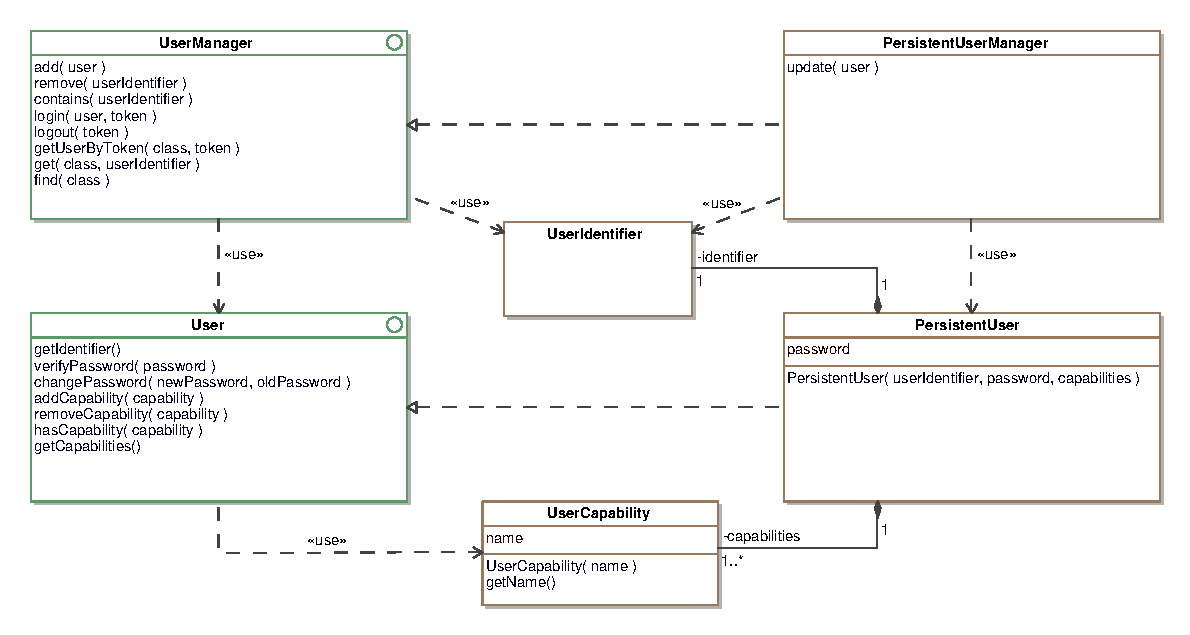
\includegraphics[width=1.0\textwidth]{images/User_Overview.eps}
	\label{user_overview}
	\caption{User - Class Overview}
\end{figure}

\subsection*{UserCapabilities}
Capabilities in conjunction with a \code{HasCapabilityTag} (Section \ref{spring}) can be used to change the appearance of a View, depending on a users status.
For example, a View for a user having an ``administrator'' capability may display different content, for example delete buttons, than for a user not having that capability.
Thus, capabilities allow for flexibility and assist in code reuse, when designing the View.
%Extensibility is achieved by using capabilities in conjunction with the \code{Has, which are aggregated by \code{User}s.

\subsection*{Login}
To reduce code repetition, \salespoint{} contains code to automate user log in.
Using a JSP template, a special login form is generated, which is handled by an interceptor.\footnote{An interceptor is a Spring concept.}
The interceptor verifies the user password and associates the current session with the user using \code{login} and \code{logoff}.
The session is required, because multiple users can be logged on at the same time.\\

To modify the content of the View, depending on whether a user is logged in or not, the \code{LoggedInTag} can be used.
